% Inbuilt themes in beamer
\documentclass[aspectratio=169]{beamer}
\usepackage{graphicx}
% Theme choice:
\usetheme{CambridgeUS}

% Title page details: 
\title{Chapter 4: Supply and Demand} 
\author{Yingfei Mu \\
    Discussion section 4}
\date{Feb, 2023}

\begin{document}

% Title page
\begin{frame}
    \titlepage 
\end{frame}

\begin{frame}{Few Reminders}
    \begin{itemize}
        \item Homework 1 is due today at \textbf{midnight}.
        \vspace{5mm}
        \item OH are usually held in Wyman S623 on Thursdays from 3-4pm unless othewise noted via Canvas.
    \end{itemize}
\end{frame}

% Outline frame
\begin{frame}{Outline}
    These slides will introduce the critical concepts of supply and demand: the behavior of firms and individuals as they interact in competitive markets.
    
    \medskip

    We will see how these two forces interact to determine prices.
\end{frame}

\begin{frame}{Supply and Demand}
    \begin{itemize}
        \item Key Concepts:
        \vspace{5mm}
        \begin{enumerate}
            \item<1-> \textbf{market}: \onslide<2->{a group of buyers and sellers of a particular good or service.}
            \vspace{5mm}
            \item<3-> \textbf{competitive market}: \onslide<4>{a market in which there are many buyers and many sellers so that each has a negligible impact on the market price.}
        \end{enumerate}
    \end{itemize}
    
\end{frame}

\begin{frame}{Perfectly competitive markets}
    In a perfectly competitive market:
    \begin{enumerate}
        \item All goods are identical
        \item No buyer or seller has influence over the market price
        \item All actors are \textit{price-takers}
    \end{enumerate}
\end{frame}

\begin{frame}{Onto Demand}
    \begin{itemize}
        \item This is the side of the market we most often find ourselves on as consumers.
        \vspace{5mm}
        \item Demand is always downward sloping, so if your mind goes blank trying to draw supply and demand, demand starts with D and so does downward!
    \end{itemize}
    \vspace{5mm}
    \begin{block}{\textbf{Law of Demand}}
        All else being equal (ceritus paribus), the \textit{quantity demanded} of a good falls when the price of a good rises.
    \end{block}
\end{frame}

\begin{frame}{Shifters of Demand}
    \begin{enumerate}
        \item<1-> Income
        \item<2-> Price of Related Goods
        \item<3-> Tastes
        \item<4-> Expectations
        \item<5-> Number of Buyers
    \end{enumerate}
    \vspace{5mm}
    \begin{itemize}
        \item<6-> All of these can shift demand in either direction (up or down). TRIBES is the way Professor Husain presents it to make it eaiser to remember, do which ever works for you.
    \end{itemize}
\end{frame}


% How people make decisions

\begin{frame}
    \frametitle{Demand schedule and curve}
    \centering
    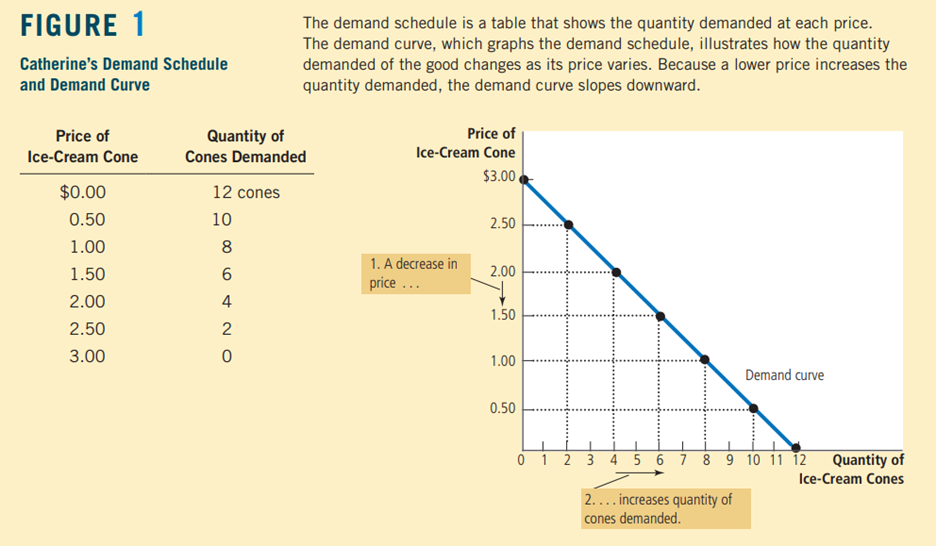
\includegraphics[width = 0.5\textwidth,keepaspectratio]{demand_curve.png}
\end{frame}

\begin{frame}{Market demand}
    The previous example showed the demand curve for one individual. The \textit{market demand} is the summation of demand curves across all individuals in a market.

    \medskip

    Demand curves are not fixed in time; many things might cause a demand curve to increase or decrease. 

    \medskip

    If demand increases when incomes increase, a good is a \textit{normal good}. If demand falls when incomes decrease, a good is an \textit{inferior good}. What are some examples of both?
\end{frame}

\begin{frame}{Complements and substitutes}
    If two goods go well together, they are \textit{complements}.

    \medskip

    If two goods fulfill the same purpose, or class, they are \textit{substitutes}.

    \medskip

    What are some examples of each?

    \medskip

    If goods A and B are complements, what will happen to demand for good B if the price of good A falls? What if they are substitutes?
\end{frame}

\begin{frame}{Example}
    Last year Maryland passed a gas tax holiday, temporarily lowering the price of gasoline. Some critics said that lowering the tax would make people want to buy more gasoline and might end up actually \textit{increasing} the price.

    \begin{enumerate}
        \item Will the tax decrease cause the demand curve for gasoline to shift?
        \item What are some complements and what are some substitutes for gasoline?
        \item What are some factors that might cause the demand curve for gasoline to shift?
    \end{enumerate}

    Does it seem plausible that the tax increase could cause the price of gasoline to go up?

  \end{frame}

  \begin{frame}{Supply}
    Now we'll talk about the other side of the market: \textit{supply}.

    \medskip

    There are lots of similarities between the two:
    \begin{itemize}
        \item \textit{Quantity supplied} is amount sellers are willing and able to sell
        \item \textit{Law of supply} governs the relationship between price and quantity supplied
        \item Supply schedules and supply curves
        \item Market supply
    \end{itemize}
\end{frame}

\begin{frame}{Shifts in supply curve}
   Just as with demand, we need to distinguish between movements along a supply curve and a shift in the curve itself

   \medskip

   What are some variables that could shift the supply curve?
\end{frame}

\begin{frame}{Shifts in supply curve}
    Just as with demand, we need to distinguish between movements along a supply curve and a shift in the curve itself

   \medskip
   
   What are some variables that could shift the supply curve?
    
    \begin{enumerate}
        \item Technology
        \item Expectations
        \item Number of sellers
    \end{enumerate}
 \end{frame}

 \begin{frame}{Equilibrium}
    Economists are generally interested in the point at which the supply and demand is balanced: \textit{equilibrium}.
    \begin{itemize}
        \item Equilibrium price (\textit{market-clearing})
        \item Equilibrium quantity
    \end{itemize}

    At this point:
    $$
    Q_D = Q_S
    $$
\end{frame}

\begin{frame}{Equilibrium}
    The actions of individuals in the market will naturally bring it into equilibrium: the \textit{law of supply and demand}.
    \begin{itemize}
        \item If there is excess supply there is a \textit{surplus}
        \item If there is excess demand there is a \textit{shortage}
    \end{itemize}

    Think about both situations:
    \begin{enumerate}
        \item What is the relationship between quantity demanded and quantity supplied?
        \item Is the price above or below equilibrium?
    \end{enumerate}
\end{frame}

\begin{frame}{Market for gasoline}
    Let's return to our question about gasoline, and run through some different scenarios.

    \medskip

    Draw supply and demand curves for the market of gasoline, and show the impact of the decrease in the gas tax.

    \medskip

    Does this represent a change in the demand curve or the supply curve?
\end{frame}

\begin{frame}
    \frametitle{Market for gasoline}
    \centering
    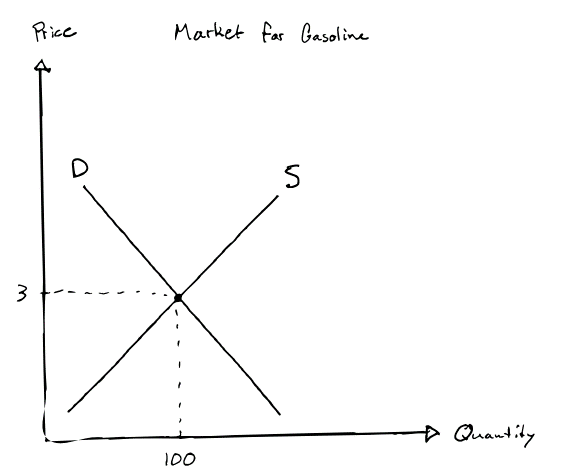
\includegraphics[width = 0.5\textwidth,keepaspectratio]{market_for_gas.png}
\end{frame}

\begin{frame}
    \frametitle{Market for gasoline}
    \centering
    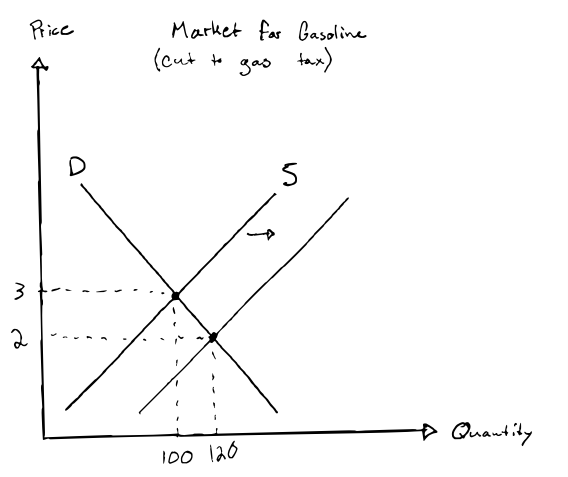
\includegraphics[width = 0.5\textwidth,keepaspectratio]{tax_cut.png}
\end{frame}

\begin{frame}{Market for gasoline}
    The tax cut caused the supply curve to shift to the right: for any given price, sellers with supply a larger quantity at a lower price.

    \medskip

    Now suppose all cars experience a sudden increase in fuel efficiency: we can drive more miles with the same amount of gasoline.

    \medskip

    Represent this as a shift in supply or demand in our market for gasoline.
\end{frame}

\begin{frame}
    \frametitle{Market for gasoline}
    \centering
    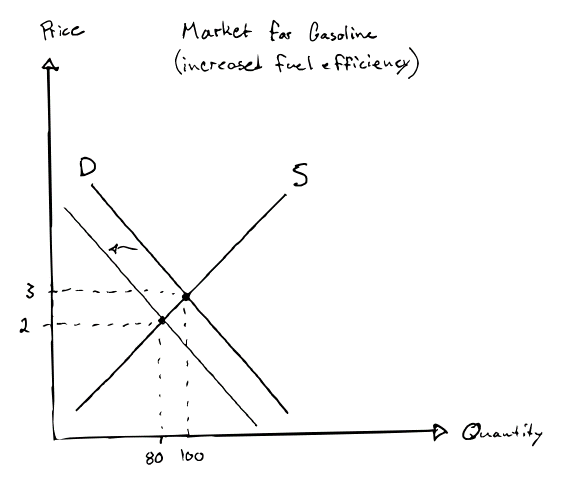
\includegraphics[width = 0.5\textwidth,keepaspectratio]{increase_efficiency.png}
\end{frame}

\begin{frame}{Market for gasoline}
    Increased fuel efficiency shifts our demand curve to the left; at any given price, we buy less gasoline than before, at a lower price.

    \medskip

    Now think about the two changes together; the gasoline tax is lowered, and fuel efficiency is increased. 
    
    \medskip

    What is the net effect on the equilibrium quantity and price? Is it unambiguous?
\end{frame}

\begin{frame}
    \frametitle{Market for gasoline}
    \centering
    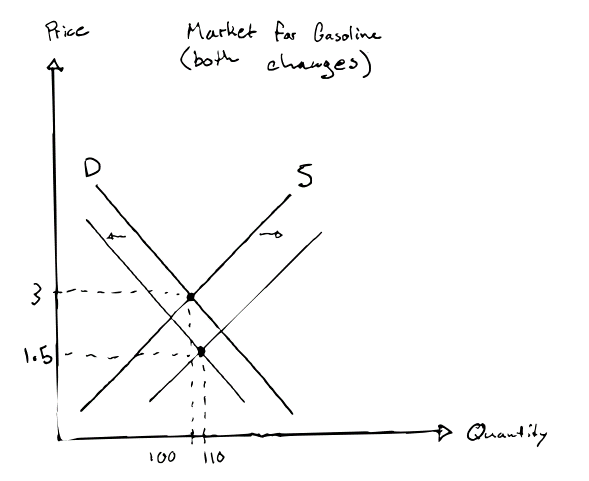
\includegraphics[width = 0.5\textwidth,keepaspectratio]{both_changes_1a.png}
\end{frame}

\begin{frame}
    \frametitle{Market for gasoline}
    \centering
    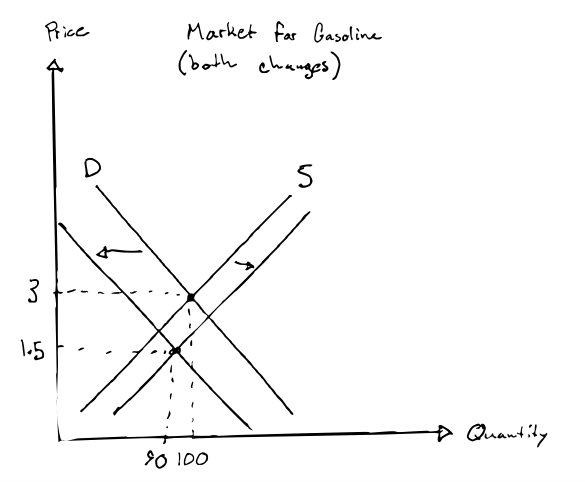
\includegraphics[width = 0.5\textwidth,keepaspectratio]{both_changes_1b.png}
\end{frame}

\begin{frame}{Market for gasoline}
    The supply curve shifts to the right, and the demand curve shifts to the left:
    \begin{itemize}
        \item The equilibrium price is unambiguously lower
        \item The equilibrium quantity may increase or decrease; it depends on the magnitude of the two shifts!
    \end{itemize}

    Note that this falls right out of our supply and demand side analyses!
    \begin{itemize}
        \item In both cases, the price decreased
        \item With the tax cut, quantity increased, but with the fuel efficiency increase, quantity decreased
    \end{itemize}

    Now suppose fuel efficiency suddenly gets \textit{worse}.

\end{frame}

\begin{frame}
    \frametitle{Market for gasoline}
    \centering
    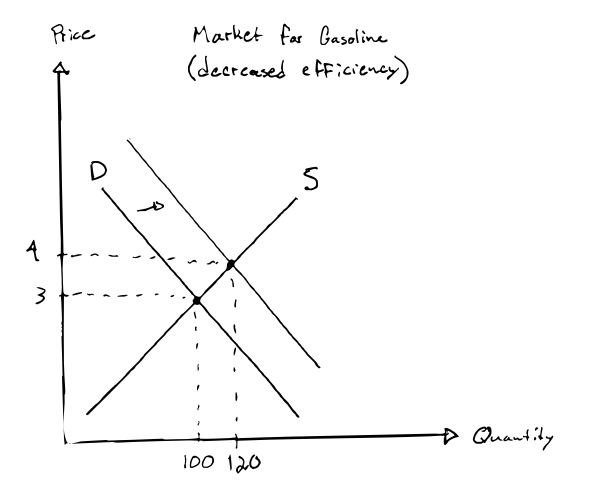
\includegraphics[width = 0.5\textwidth,keepaspectratio]{decrease_efficiency.png}
\end{frame}

\begin{frame}{Market for gasoline}
    The effect is the opposite as before: decreased fuel efficiency shifts our demand curve to the right; at any given price, we buy more gasoline than before, at a higher price.

    \medskip

    Now think about the two changes together; the gasoline tax is lowered, and fuel efficiency is decreased. 
    
    \medskip

    What are the net effects on the equilibrium quantity and price?
\end{frame}

\begin{frame}
    \frametitle{Market for gasoline}
    \centering
    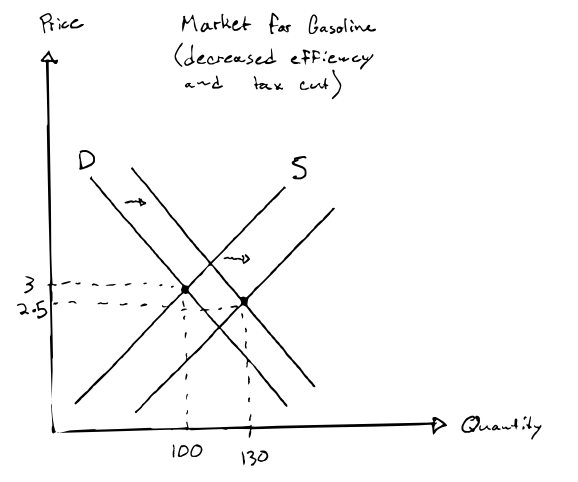
\includegraphics[width = 0.5\textwidth,keepaspectratio]{both_changes_2a.png}
\end{frame}

\begin{frame}
    \frametitle{Market for gasoline}
    \centering
    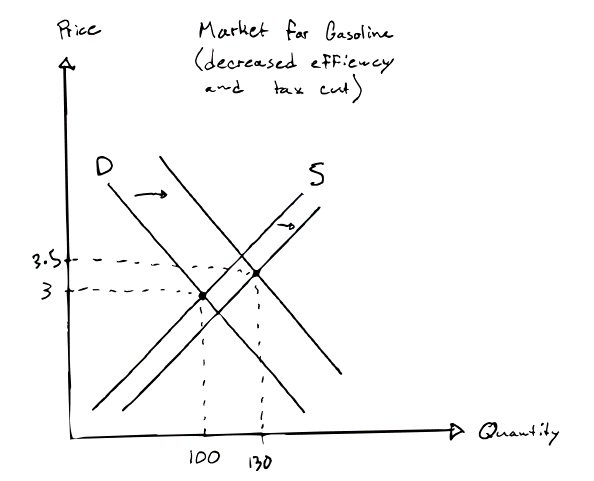
\includegraphics[width = 0.5\textwidth,keepaspectratio]{both_changes_2b.png}
\end{frame}

\begin{frame}{Market for gasoline}
    Supply and demand curves both shift to the right:
    \begin{itemize}
        \item The equilibrium quantity is unambiguously higher
        \item The equilibrium price may increase or decrease; it depends on the magnitude of the two shifts!
    \end{itemize}

    Again, we can get this right from our supply and demand side analyses:
    \begin{itemize}
        \item In both cases, the quantity increased
        \item With the tax cut, price decreased, but with the fuel efficiency decrease, price increased
        \item Net effect on price is ambiguous 
    \end{itemize}

\end{frame}

\begin{frame}{Market for Orioles tickets}
    In the last few years, the Orioles have gone from one of the worst teams in MLB to one of the best.

    \begin{enumerate}
        \item Draw the supply and demand curves for Orioles tickets.
        \item Does the supply curve look like it did in the gasoline market?
        \item Will the team's improved record effect supply or demand, and why?
        \item What will happen to equilibrium price and quantity?
    \end{enumerate}
\end{frame}

\begin{frame}
    \frametitle{Market for Orioles tickets}
    \centering
    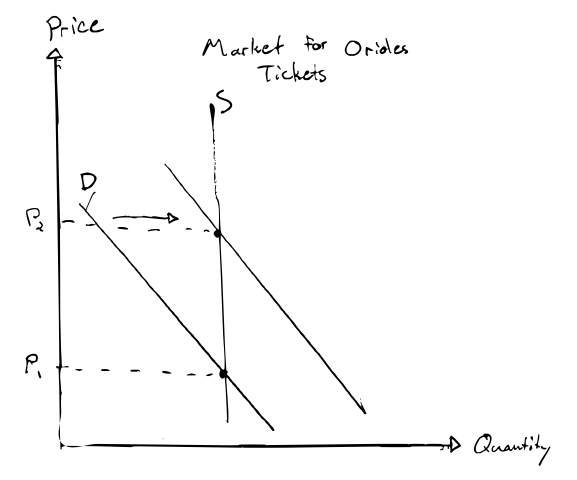
\includegraphics[width = 0.5\textwidth,keepaspectratio]{orioles.png}
\end{frame}

\begin{frame}{Market for Orioles tickets}
    \begin{itemize}
        \item Supply curve is vertical: why?
        \item A better team means more fans want to attend more games, shifting the demand curve to the right
        \item The equilibrium quantity is the same, but the price has increased
    \end{itemize}

    Is this a realistic way to think about the market for tickets?
\end{frame}

\begin{frame}{Market for Orioles tickets}
    Is this a realistic way to think about the ticket market?
    \begin{itemize}
        \item In some ways: we really do see ticket prices increasing, and the number of seats really is fixed
        \item In reality, not all seats are the same (different markets?) and not all seats get sold (there are fixed costs and frictions)
        \item Don't worry about any of this for now!
    \end{itemize}
\end{frame}

\end{document}